\documentclass[pdf]{beamer}
\mode<presentation>{} 

\usepackage{hyperref}
\usepackage{pgf}
\usepackage{tikz}
\usetikzlibrary{trees}
\usetikzlibrary{arrows,automata}
\usetikzlibrary{automata,positioning}
\usetikzlibrary{shapes}
\usepackage{tikz-qtree,tikz-qtree-compat}
\usepackage{mathtools,enumerate,amssymb}
\usepackage[utf8]{inputenc}
\usepackage[T1]{fontenc}
\usepackage{graphicx}
\usepackage{wrapfig}
\usepackage[export]{adjustbox}
\definecolor{Blue}{RGB}{0,0,100}
\definecolor{background}{RGB}{255,255,204}

\title{Task-Centered System Design}
\subtitle{Human Computer Interaction}
\AtBeginSection[]{}

\setbeamertemplate{sidebar right}{}
\setbeamertemplate{footline}{%
\hfill\usebeamertemplate***{navigation symbols}
\hspace{1cm}\insertframenumber{}/\inserttotalframenumber}

\graphicspath{{./img/}}



\begin{document}



\definecolor{myBlue}{RGB}{0,0,100}
\definecolor{background}{RGB}{255,255,255}

{\setbeamercolor{background canvas}{bg=background}
\begin{frame}
\vspace{10mm}
\huge{\raggedleft{\color{black}{\textbf{Task-Centered System Design}}}}

\large{\raggedleft{\color{black} Human Computer Interaction}}

\begin{flushright}
\end{flushright}

\fontsize{7pt}{1pt}\selectfont{
Based on slide deck 

\textbf{Part 2: Understanding users and their tasks. Task-Centered System Design}

Human Computer Interaction I: Principles and Design

by

\textbf{Saul Greenberg}
\newline
Professor
\newline
\textbf{University of Calgary, Canada}

\textit{The new slides are marked with a *}
}

\fontsize{5pt}{1pt}\selectfont{ \textcolor{lightgray}
{Slide deck by Saul Greenberg. Permission is granted to use this for non-commercial purposes as long as general credit to Saul Greenberg is clearly maintained.
Warning: some material in this deck is used from other sources without permission. Credit to the original source is given if it is known.}}

\end{frame}}



% Inaintea codului fiecarui slide se vor scrie urmatoarele informatii:
% Nume si prenume student
% Numarul slide-ului corespunzator din prezentarea prof. Saul Greenberg
% Numele imaginilor inserate trebuie sa fie numar_slide_nume_imagine.extensie_imagine

% Deaconescu Andrei Eduard
%slide 1
\begin{frame}

\begin{itemize}
	\item[] {\textbf {\LARGE Task-Centered System Design}} \newline
	\item [] How to develop task examples			
    \item [] How to evaluate designs via task-centered walkthroughs
    \item [] Exercise: The Cheap Shop interface
\end{itemize}
\end{frame}



% Deaconescu Andrei Eduard
%slide 2
\begin{frame}
\vspace{8mm}
\textcolor{myBlue}{\textbf{\Large{The Cheap Shop Catalog Store}}}

\textcolor{red}{\rule{10cm}{1mm}}

    \begin{itemize}
	\item []In Cheap Shop, people shop by\\ browsing paper catalogs scattered \\ around the store.\newline		
	\item[]When people see an item they want,\\ they enter its item code from\\ the catalog onto a form.\newline 
    \item[]People give this form to a clerk, who\\ brings the item(s) from the back\\ room to the front counter. \newline
    \item[]People then pay for the items they \\ want.
	
	\end{itemize}
    
    \begin{picture}(0,0)
      \put(200,95){\hbox{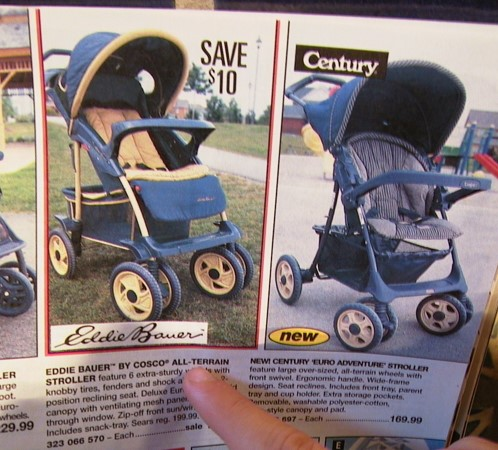
\includegraphics[scale=0.5]{1_Picture1.jpg}}}      
  	\end{picture}
    
    \begin{picture}(0,0)
      \put(205,20){\hbox{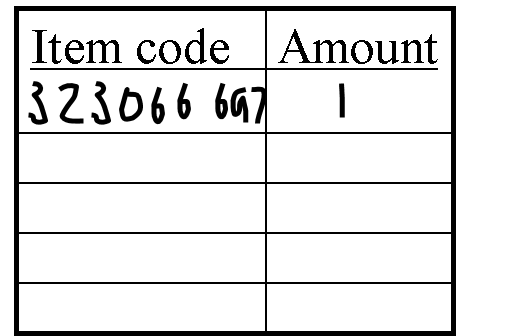
\includegraphics[scale=0.5]{1_Picture2.png}}}      
  	\end{picture}
\bigskip \bigskip \bigskip \bigskip \bigskip \bigskip
\leavevmode\makebox(0,0){\put(280,0){\tiny{\textcolor{gray}{Saul Greenberg}}}}
\end{frame}    



% Deaconescu Andrei Eduard
%slide 3
\begin{frame}
\begin{wrapfigure}{r}{0.7\textwidth}
\vspace*{-32mm}
    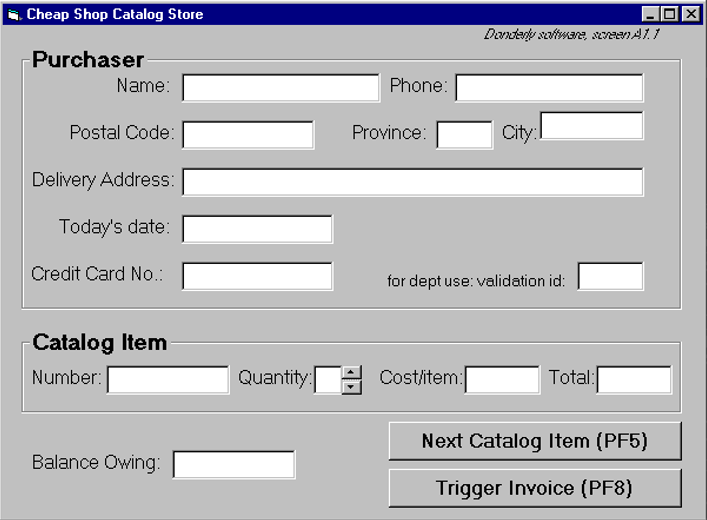
\includegraphics[width=0.7\textwidth]{28_Screen1.png} \par
    \vspace{3mm}
   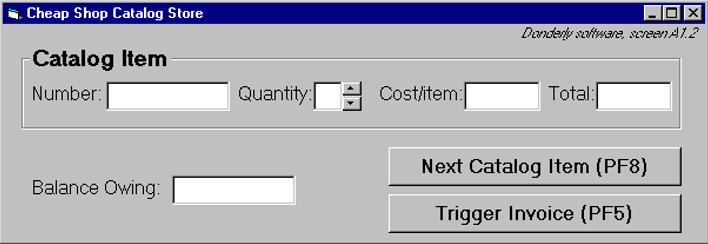
\includegraphics[width=0.7\textwidth]{28_Screen2.png}  
\end{wrapfigure}
\frametitle{\textcolor{myBlue}{\textbf{\hspace{5mm}{Cheap Shop}}}} \par
\vspace{10mm}
\textcolor{myBlue}{\footnotesize{{\hspace{15mm}{Screen 1}}}}\par
\vspace{40mm}
\textcolor{myBlue}{\footnotesize{{\hspace{15mm}{Screen 2}}}}
\end{frame}



% Deaconescu Andrei Eduard
%slide 4
\begin{frame}
\vspace{8mm}
\textcolor{myBlue}{\textbf{\Large{Seat-of-your-pants interface design}}}

\textcolor{red}{\rule{10cm}{1mm}}	
	
    Is this a good or a bad interface? 
    \begin{itemize}
      \item [--]do you go by gut feel?
      \item [--]do you go by how it looks?
      \item [--]do you judge it by familiarity to other interfaces?
      \item [--]if there are problems, are they minor or serious?
      \item [--]did you miss anything that you really shouldn’t have?
      \item [--]is your opinion correct? 
      \item [--]how can you tell? \newline
    \end{itemize}
    
    Alternative: are there methods where you can:
    \begin{itemize}
      \item [--]systematically determine if this interface matches the needs of its end users?
      \item [--]systematically discover the usability bugs?   
    \end{itemize}
\end{frame}



% Deaconescu Andrei Eduard
%slide 5
\begin{frame}
\vspace{8mm}
\textcolor{myBlue}{\textbf{\Large{Requirements analysis}}}

\textcolor{red}{\rule{10cm}{1mm}}	

A software perspective
    \begin{itemize}
      \item [--]exactly what functions should the system have?      
    \end{itemize}
    
	\begin{minipage}[t]{0.28\linewidth}  
      \bigskip
      
\includegraphics[scale=0.5]{5_Picture5.png}
  	\end{minipage}
\hfill
\begin{minipage}[t]{0.65\linewidth}   
\bigskip
\bigskip
\bigskip
\bigskip
\bigskip
\LARGE \textbf{The User} \newline
\normalsize{person who will mould \newline themselves to fit your system}
\end{minipage}           
\end{frame}



% Deaconescu Andrei Eduard
%slide 6
\begin{frame}
\vspace{8mm}
\textcolor{myBlue}{\textbf{\Large{Requirements analysis}}}

\textcolor{red}{\rule{10cm}{1mm}}	

An end-users perspective
    \begin{itemize}
      \item [--]exactly who would use the system to do exactly what?     
    \end{itemize}
    
	\begin{minipage}[t]{0.28\linewidth}  
      \bigskip
      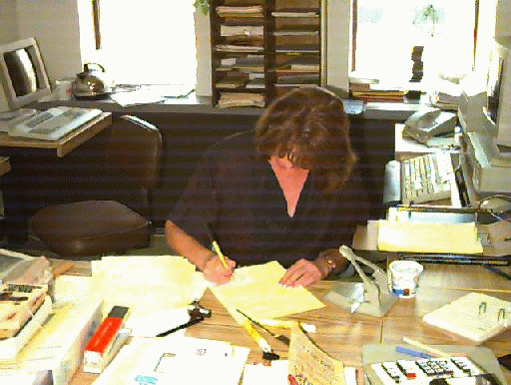
\includegraphics[scale=0.5]{6_Picture6.png}
  	\end{minipage}
\hfill
\begin{minipage}[t]{0.57\linewidth}   
\bigskip
\bigskip
\bigskip
\bigskip
\LARGE \textbf{Mary Franklin} \newline
\normalsize{a real person with real\newline constraints trying to get her\newline job done}
\end{minipage}           
\end{frame}



% Deaconescu Andrei Eduard
%slide 7
\begin{frame}
\vspace{8mm}
\textcolor{myBlue}{\textbf{\Large{Task-Centered System Design}}}

\textcolor{red}{\rule{10cm}{1mm}}	

An end-users perspective
    \begin{itemize}
      \item [--]exactly who would use the system to do exactly what?   
    \end{itemize}  
    
 \textbf{Phases:}
 \begin{enumerate}[\color{black} 1]
 \item \textbf{Identification}
 	\begin{itemize}
      \item []identify \textbf{\textit{specific users}} and articulate their \textbf{\textit{concrete tasks}}
    \end{itemize} 
 \item \textbf{Requirements}
 	\begin{itemize}
      \item []decide which of these tasks and users the design will support
    \end{itemize} 
 \item \textbf{Design}
 	\begin{itemize}
      \item []base design representation and dialog sequences on these tasks  
    \end{itemize} 
 \item \textbf{Walkthrough Evaluations}
 	\begin{itemize}
      \item []using your design, walk through these tasks to test the interface
    \end{itemize} 
 \end{enumerate}
\end{frame}



% Deaconescu Andrei Eduard
%slide 8
\begin{frame}
\vspace{8mm}
\textcolor{myBlue}{\textbf{\Large{Foreshadowing ...}}}

\textcolor{red}{\rule{10cm}{1mm}}	


     \textbf{Task example 1}
     \bigskip
     \begin{itemize}
        \item[\textcolor{black}{--}] Fred Johnson, who is caring for his demanding toddler son, wants a good quality umbrella stroller (red is preferred, but blue is acceptable). 
        \bigskip
        \item[\textcolor{black}{--}] He browses the catalog and chooses the JPG stroller (cost \$98. item code 323 066 697).
        \bigskip
        \item[\textcolor{black}{--}] He pays for it in cash, and uses it immediately.
        \bigskip
        \item[\textcolor{black}{--}] Fred is a first-time customer to this store, has little computer experience, and says he types very slowly with one finger. He lives nearby on Dear Bottom Avenue NW.


     \end{itemize}
     \begin{figure}[b]
    	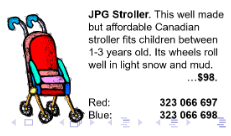
\includegraphics[scale = 0.7, right]{8_Picture1.png}
    \end{figure}
\end{frame}



% Dumitrache Cezar Adrian
% slide 9
\begin{frame}
\vspace{8mm}
\textcolor{myBlue}{\textbf{\Large{Foreshadowing ...}}}

\textcolor{red}{\rule{10cm}{1mm}}	

     \section{introduction}
     \textbf{Discussion}
     \bigskip
	 \begin{itemize}
        \item[\textcolor{black}{--}] Fred has many properties of our typical expected user:
		\begin{itemize}
            \item[{$\bullet$}]many customers are first time shoppers
			\item[{$\bullet$}]a good number have no computer experience
            \item[{$\bullet$}]a good number are poor typists
		\end{itemize}
        \bigskip
        \item[\textcolor{black}{--}] The task type is routine and important.
        \begin{itemize}
            \item[{$\bullet$}]many people often purchase only one item
			\item[{$\bullet$}]a good number of those pay by cash
            \item[{$\bullet$}]as with Fred, people often have a general sense of what they want to buy, but decide on the actual product only after seeing what is available
		\end{itemize}
     \end{itemize}
        
\end{frame}



% Dumitrache Cezar Adrian
% slide 10
\begin{frame}
\vspace{8mm}
\textcolor{myBlue}{\textbf{\Large{Phase 1: Identify users + tasks}}}

\textcolor{red}{\rule{10cm}{1mm}}	

Get in touch with real people who will be

potential users of your system
\begin{itemize}
         \item[{$\bullet$}]prototypical categories
         \item[{$\bullet$}]extremes
\end{itemize}       

		\begin{picture}(0,0)
      	\put(225,-20){\hbox{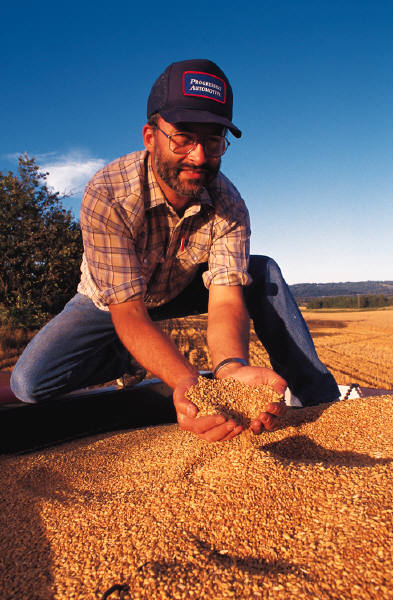
\includegraphics[scale=0.4]{2_Picture1.jpg}}}      
  		\end{picture}
    
   	    \begin{picture}(0,0)
        \put(225,-120){\hbox{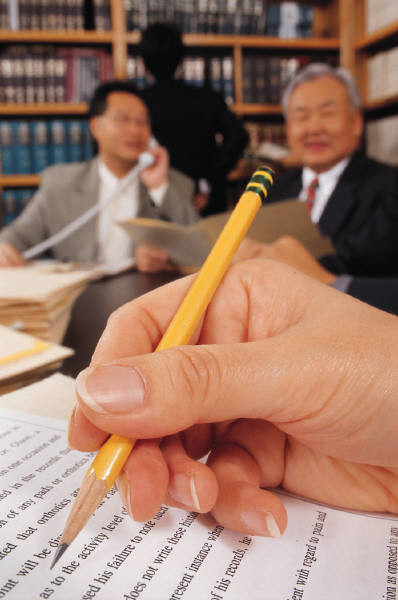
\includegraphics[scale=0.4]{2_Picture2.jpg}}}      
  	    \end{picture}
Learn about their real tasks
	 \begin{itemize}
	    \item[\textcolor{black}{--}]articulate \textbf{concrete}, \textbf{detailed} examples of 

tasks they perform or want to perform 

that your system should support	
	   \begin{itemize}
		 \item[{$\bullet$}]routine
		 \item[{$\bullet$}]infrequent but important
         \item[{$\bullet$}]infrequent and incidental
		\end{itemize}
        \end{itemize}
        		
\end{frame}



% Dumitrache Cezar Adrian
% slide 11
\begin{frame}
\vspace{8mm}
\textcolor{myBlue}{\textbf{\Large{Phase 1: Identify users + tasks}}}

\textcolor{red}{\rule{10cm}{1mm}}	

\begin{itemize}
	\item[]  {\LARGE How do you identify tasks?} \newline
	\item [] {\textbf{Immerse yourself in a real person’s environment}}		
    \item [] \textbf{Observe} people in their actual work context
    \item [] \textbf{Interview} people as they do their work
    \item [] \textbf{Shadow} a person over the course of his or her day
    \item [] \textbf {Serve} people's requests
    \item [] \textbf ...
\end{itemize}
\end{frame}



% Dumitrache Cezar Adrian
% slide 12
\begin{frame}
\vspace{8mm}
\textcolor{myBlue}{\textbf{\Large{Phase 1: Identify users + tasks}}}

\textcolor{red}{\rule{10cm}{1mm}}	

\begin{itemize}
	\item[]  {\LARGE If there are no real users or tasks…} \newline
	 \item[\textcolor{black}{--}]think again, there probably are!

		\begin{picture}(0,0)
      	\put(225,-10){\hbox{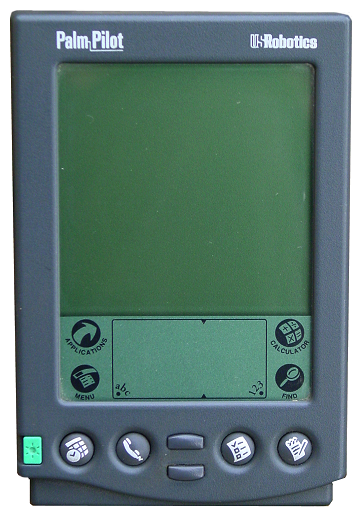
\includegraphics[scale=0.2]{palmpilot.png}}}      
  		\end{picture}	 
	 
     \bigskip
    \item [] Jeff Hawkins, the inventor of the Palm Pilot, was said to
have carried a small block of wood around in his shirt pocket … As various everyday situations arose, he would take out the block of wood and imagine how he would use the device.
	\bigskip
    \bigskip
    \item [] The same technique can be used to evoke a response from expected end-users
   
\end{itemize}
\end{frame}



% Dumitrache Cezar Adrian
% slide 13
\begin{frame}
\vspace{8mm}
\textcolor{myBlue}{\textbf{\Large{Phase 1: Identify users + tasks}}}

\textcolor{red}{\rule{10cm}{1mm}}	

\begin{itemize}
	\item[]  {\LARGE If all else fails…} \newline
	 \item[\textcolor{black}{--}]describe your expected set of users
     \item[\textcolor{black}{--}]describe your expected set of tasks
\end{itemize}
\begin{itemize}
	\item[]  {\LARGE These will become your ‘assumed users and tasks’} \newline
	 \item[\textcolor{black}{--}]verify them later as information comes in
     \item[\textcolor{black}{--}]modify them as needed
\end{itemize}

\end{frame}



% Dumitrache Cezar Adrian
% slide 14
\begin{frame}
\vspace{8mm}
\textcolor{myBlue}{\textbf{\Large{Phase 1: Developing good task examples}}}

\textcolor{red}{\rule{10cm}{1mm}}	

\begin{itemize}
	\item[]  {\LARGE 1.Says what the user wants to do but does not say how they would do it} \newline
	 \item[\textcolor{black}{--}]no assumptions made about the interface
     \item[\textcolor{black}{--}]can be used to compare design alternatives in a fair way
\end{itemize}
\begin{itemize}
	\item[]  {\LARGE 2. Are very specific} \newline
	 \item[\textcolor{black}{--}]says exactly what the user wants to do
     \item[\textcolor{black}{--}]specifies actual items the user would somehow want to input
\end{itemize}

\end{frame}



% Dumitrache Cezar Adrian
% slide 15
\begin{frame}
\vspace{8mm}
\textcolor{myBlue}{\textbf{\Large{Phase 1: Developing good task examples}}}

\textcolor{red}{\rule{10cm}{1mm}}	

\begin{itemize}
	\item[]  {\LARGE 3. Describes a complete job} \newline
	 \item[\textcolor{black}{--}]forces designer to consider how interface features work together
     \item[\textcolor{black}{--}]contrasts how information input / output flows through the dialog
     \begin{itemize}
      \item[{$\bullet$}]where does information come from?
      \item[{$\bullet$}]where does it go?
      \item[{$\bullet$}]what has to happen next?
     \end{itemize}
    \item[] {Do not}
    \begin{itemize}
    \item[{$\bullet$}]create a list of simple things the system should do
    \item[{$\bullet$}]present a sub-goal independent of other sub-goals
    \end{itemize}
\end{itemize}
\end{frame}



% Dumitrache Cezar Adrian
% slide 16
\begin{frame}
\vspace{8mm}
\textcolor{myBlue}{\textbf{\Large{Phase 1: Developing good task examples}}}

\textcolor{red}{\rule{10cm}{1mm}}	

\begin{itemize}
	\item[]  {\LARGE 4. Says who the users are} \newline
	 \item[\textcolor{black}{--}]name names, if possible
     \item[\textcolor{black}{--}]says what they know
     \bigskip
     \bigskip
     \item[\textcolor{black}{--}]Why?
      \begin{itemize}
      \item[{$\bullet$}]design success strongly influenced by what users know
      \item[{$\bullet$}]can go back and ask them questions later
      \item[{$\bullet$}]reflects real interests of real users
      \item[{$\bullet$}]helps you find tasks that illustrate functionality in that person’s real work context
     \end{itemize}
     \end{itemize}
\end{frame}


        
% Florescu Constantin-Emanuel
% slide 17
{%\setbeamercolor{background canvas}{bg=background}
\setbeamercolor{normal text}{fg=Blue}
\usebeamercolor[fg]{normal text}
\begin{frame}{}
	\vspace{8mm}
	\textcolor{Blue}{\textbf{\Large{Phase 1: Developing good task examples}}}
    \textcolor{red}{\rule{10cm}{1mm}}

    5. Are evaluated
        \begin{itemize}
        \item [\textcolor{Blue}{--}] Circulate description to users, and rewrite if needed
            \begin{itemize}
            \item[{$\bullet$}] ask users for
                  \begin{itemize}
                      \item[{--}] omissions
                      \item[{--}] corrections
                      \item[{--}] clarifications
                      \item[{--}] suggestions
                  \end{itemize}
            \end{itemize}
        \end{itemize}

    \bigskip
    \bigskip
     6. As a set, identifies a broad coverage of users and task types
    \begin{tabular}{ll}
    {--}  the typical 'expected' user & typical routine tasks \\
    {--}  the occasional but important user & intrequent but important tasks \\
    {--}  the unusual user, & unexpected or odd tasks \\
    \end{tabular}

\end{frame}}



% Florescu Constantin-Emanuel
% slide 18
{
%\setbeamercolor{background canvas}{bg=background}
\setbeamercolor{normal text}{fg=Blue}
\usebeamercolor[fg]{normal text}
\begin{frame}
	\vspace{8mm}
	\textcolor{Blue}{\textbf{\Large{Phase 2: Requirements}}}
    \textcolor{red}{\rule{10cm}{1mm}}


    \bigskip
     Which user types will be addressed by the interface?
        \begin{itemize}
        \item[{--}] designs can rarely handle everyone!
        \item[{--}] includes why particular users are included / excluded
        \end{itemize}

    \bigskip
     Which tasks will be addressed by the interface?
        \begin{itemize}
        \item[{--}] designs can rarely handle all tasks
        \item[{--}] requirements listed in terms of how they address tasks
            \begin{itemize}
                \item[{$\bullet$}] Absolutely must include:
                \item[{$\bullet$}] Should include:
                \item[{$\bullet$}] Could include:
                \item[{$\bullet$}] Exclude:
            \end{itemize}

    \bigskip

        \item[{--}] Discussion includes why items are in those categories
        \end{itemize}

\end{frame}}


% Florescu Constantin-Emanuel
% slide 19
{
%\setbeamercolor{background canvas}{bg=background}
\setbeamercolor{normal text}{fg=Blue}
\usebeamercolor[fg]{normal text}
\begin{frame}
	\vspace{8mm}
	\textcolor{Blue}{\textbf{\Large{Phase 3: Design as Scenarios}}}
    \textcolor{red}{\rule{10cm}{1mm}}


    \bigskip
     Develop design to fit users and specific tasks
        \begin{itemize}

        \item[{--}] ground interfaces in reality

        \end{itemize}

    \bigskip
     Use tasks to
        \begin{itemize}
        \item[{--}] get specific about possible designs
        \item[{--}] consider the real world contexts of real users
        \item[{--}] consider how design features work together
            \begin{itemize}
                \item[{$\bullet$}] what would the user do / see step-by-step when performing this task?
            \end{itemize}
        \end{itemize}

\end{frame}}



% Florescu Constantin-Emanuel
% slide 20
{%\setbeamercolor{background canvas}{bg=background}
\setbeamercolor{normal text}{fg=Blue}
\usebeamercolor[fg]{normal text}
\begin{frame}
	\vspace{8mm}
	\textcolor{Blue}{\textbf{\Large{Phase 4: Walk-through Evaluation}}}
    \textcolor{red}{\rule{10cm}{1mm}}

\bigskip
 Good for debugging an interface

\bigskip

 \textbf{Process}
 \begin{enumerate}[ 1]
 \item Select one of the task scenarios
 \item For each user's step/action in the task:
	\begin{enumerate}[ a)]
    \item can you build a believable story that motivates the user's actions?
    \item can you rely on user's expected knowledge and training about system?
    \item if you cannot:
    	\begin{itemize}
        \item[{$\bullet$}] you've located a problem in the interface!
        \item[{$\bullet$}] note the problem, including any comments
        \item[{$\bullet$}] assume it has been repaired
        \end{itemize}
    \item go to the next step in the task
    \end{enumerate}
 \end{enumerate}
\end{frame}}



% Florescu Constantin-Emanuel
% slide 21
{%\setbeamercolor{background canvas}{bg=background}
\setbeamercolor{normal text}{fg=Blue}
\usebeamercolor[fg]{normal text}
\begin{frame}
	\vspace{8mm}
	\textcolor{Blue}{\textbf{\Large{The Cheap Shop Catalog Store}}}
    \textcolor{red}{\rule{10cm}{1mm}}


\begin{wrapfigure}{r}{0.3\textwidth}
      \centering
      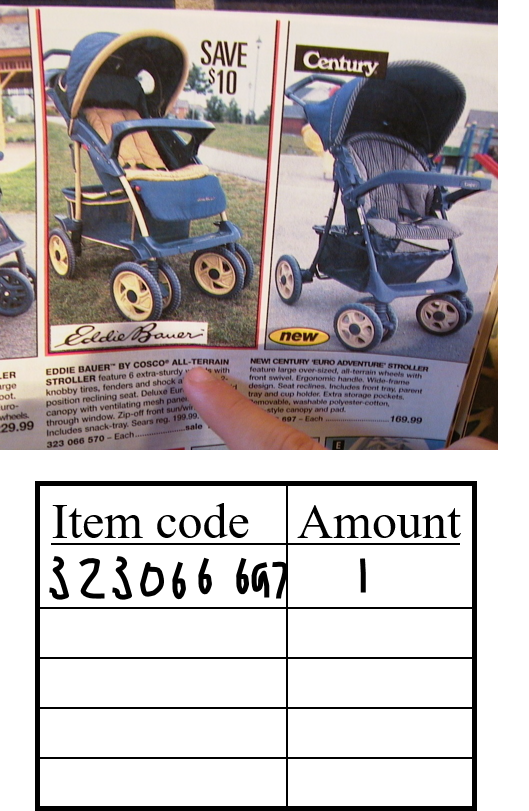
\includegraphics[scale = 0.4]{21_imagine.png}
\end{wrapfigure}
    \bigskip
    In Cheap Shop, people shop by browsing paper catalogs scattered around the store.

    \bigskip

    When people see an item they want, they enter its item code from the catalog onto a form.

    \bigskip

    People give this form to a clerk, who brings the item(s) from the back room to the front counter. 

    \bigskip

    People then pay for the items they want.

\end{frame}}

% Florescu Constantin-Emanuel
% slide 22
{%\setbeamercolor{background canvas}{bg=background}
\setbeamercolor{normal text}{fg=Blue}
\usebeamercolor[fg]{normal text}
\begin{frame}
	\vspace{8mm}
	\textcolor{Blue}{\textbf{\Large{Developing task examples: Cheap Shop}}}
    \textcolor{red}{\rule{10cm}{1mm}}


     \bigskip
     \textbf{Task example 1}
   
          \begin{itemize}
        \item[\textcolor{black}{--}] Fred Johnson, who is caring for his demanding toddler son, wants a good quality umbrella stroller (red is preferred, but blue is acceptable). 
        \bigskip
        \item[\textcolor{black}{--}] He browses the catalog and chooses the JPG stroller (cost \$98. item code 323 066 697).
        \bigskip
        \item[\textcolor{black}{--}] He pays for it in cash, and uses it immediately.
        \bigskip
        \item[\textcolor{black}{--}] Fred is a first-time customer to this store, has little computer experience, and says he types very slowly with one finger. He lives nearby on Dear Bottom Avenue NW.


     \end{itemize}
     \begin{figure}[b]
    	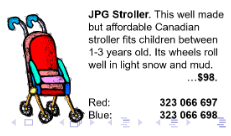
\includegraphics[scale = 0.7, right]{8_Picture1.png}
    \end{figure}
\end{frame}}



% Florescu Constantin-Emanuel
% slide 23
{%\setbeamercolor{background canvas}{bg=background}
\setbeamercolor{normal text}{fg=Blue}
\usebeamercolor[fg]{normal text}
\begin{frame}
	\vspace{8mm}
	\textcolor{Blue}{\textbf{\Large{Developing task examples: Cheap Shop}}}
    \textcolor{red}{\rule{10cm}{1mm}}


    \bigskip
    \textbf{Discussion}
    \bigskip
    \begin{itemize}
    	\item[{--}] Fred has many properties of our typical expected user:
        \begin{itemize}
        	\item[{$\bullet$}] many customers are first time shoppers,
            \item[{$\bullet$}] a good number have no computer experience
            \item[{$\bullet$}] a good number are poor typists.
        \end{itemize}
        \item[{--}] The task type is routine and important. 
        \begin{itemize}
        	\item[{$\bullet$}] many people often purchase only one item
            \item[{$\bullet$}] a good number of those pay by cash
            \item[{$\bullet$}] as with Fred, people often have a general sense of what they want to buy, but decide on the actual product only after seeing what is available.
        \end{itemize}
	\end{itemize}
\end{frame}}



% Florescu Constantin-Emanuel
% slide 24
{
%\setbeamercolor{background canvas}{bg=background}
\setbeamercolor{normal text}{fg=Blue}
\usebeamercolor[fg]{normal text}
\begin{frame}
	\vspace{8mm}
	\textcolor{Blue}{\textbf{\Large{Developing task examples: Cheap Shop}}}
    \textcolor{red}{\rule{10cm}{1mm}}


    \bigskip
    \textbf{Task example 2}
    \bigskip
    \begin{itemize}
        \item[{--}] Mary Vornushia is price-comparing the costs of a child’s bedroom set, consisting of a wooden desk, a chair, a single bed, a mattress, a bedspread, and a pillow all made by Furnons Inc.
        \item[{--}] She takes the description and total cost away with her to check against other stores.
        \item[{--}] Three hours later, she returns and decides to buy everything but the chair.
        \item[{--}] She pays by credit card.
        \item[{--}] She asks for the items to be delivered to her daughter’s home at 31247 Lucinda Drive, in the basement suite at the back of the house.
        \bigskip
        \item[{--}] Mary is elderly and arthritic.
	\end{itemize}
\end{frame}}



% Horodincă Alina-Elena
% slide 25
\definecolor{myBlue}{RGB}{0,0,100}
\definecolor{background}{RGB}{255,255,204}

{%\setbeamercolor{background canvas}{bg=background}
\begin{frame}
\frametitle{\textcolor{myBlue}{\textbf{\hspace{8mm}{Developing task examples: Cheap Shop}}}}
\vspace*{-12mm}
\textcolor{red}{\rule{10cm}{1mm}}

\vspace{3mm}
\textcolor{myBlue}{\textbf{\hspace{2mm}{Discussion}}}
\vspace{2mm}
\begin{itemize}
	\item[\textcolor{myBlue}{--}] \textcolor{myBlue}{{\small Like Mary,}}
		\begin{itemize}
			\item[\textcolor{myBlue}{$\bullet$}]\textcolor{myBlue}{{\footnotesize a reasonable number of store customers are elderly, with infirmities that inhibit their physical abilities. }}
         	\item[\textcolor{myBlue}{$\bullet$}]\textcolor{myBlue}{{\footnotesize a modest number of them also enjoy comparison shopping, perhaps because they have more time on their hands or because they are on low income. }}
		\end{itemize}    
	\vspace{5mm}
	\item[\textcolor{myBlue}{--}] \textcolor{myBlue}{{\small The task type is less frequent, but still important.}}
		\begin{itemize}
       		\item[\textcolor{myBlue}{$\bullet$}]\textcolor{myBlue}{{\footnotesize although this would be considered a ‘major’ purchase in terms of the total cost, the number of items purchased is not unusual.}}
            \item[\textcolor{myBlue}{$\bullet$}]\textcolor{myBlue}{{\footnotesize delivery of large items is the norm }}
            \item[\textcolor{myBlue}{$\bullet$}]\textcolor{myBlue}{{\footnotesize most customers pay by credit card for larger orders. }}
     	\end{itemize}
\end{itemize}
\end{frame}}



% Horodincă Alina-Elena
% slide 26
{%\setbeamercolor{background canvas}{bg=background}
\begin{frame}
\frametitle{\textcolor{myBlue}{{\textbf{\hspace{8mm}{Developing task examples: Cheap Shop}}}}}
\vspace*{-2mm}
\textcolor{red}{\rule{10cm}{1mm}}

\vspace{3mm}
\textcolor{myBlue}{\textbf{\hspace{2mm}{Task example 3}}}
\vspace{2mm}
\begin{itemize}
	\item[\textcolor{myBlue}{--}] \textcolor{myBlue}{{\small John Forham, the sole salesperson in the store, is given a list of 10 items by a customer who does not want to use the computer. }}
	\item[\textcolor{myBlue}{--}] \textcolor{myBlue}{The items are: }
		\begin{itemize}
			\item[\textcolor{myBlue}{$\bullet$}] \textcolor{myBlue}{{\footnotesize 4 pine chairs, 1 pine table, 6 blue place mats, 6 “lor” forks, 6 “lor” table spoons, 6 “lor” teaspoons, 6 “lor” knives, 1 “tot” tricycle, 1 red ball, 1 “silva” croquet set}}
		\end{itemize}  
	\item[\textcolor{myBlue}{--}] \textcolor{myBlue}{{\small After seeing the total, the customer tells John he will take all but the silverware.}}
    \item[\textcolor{myBlue}{--}] \textcolor{myBlue}{{\small The customer then decides to add 1 blue ball to the list.}}
    \item[\textcolor{myBlue}{--}] \textcolor{myBlue}{{\small The customer starts paying by credit card, but then decides to pay cash. The customer tells John he wants the items delivered to his home the day after tomorrow. While this is occurring, 6 other customers are waiting for John. }}
	\vspace{4mm}
    \item[\textcolor{myBlue}{--}]\textcolor{myBlue}{{\small John has been on staff for 1 week, and is only partway through his training program.}}
\end{itemize}
\end{frame}}



% Horodincă Alina-Elena
% slide 27
{%\setbeamercolor{background canvas}{bg=background}
\begin{frame}
\frametitle{\textcolor{myBlue}{{\textbf{\hspace{8mm}{Developing task examples: Cheap Shop}}}}}
\vspace*{-8mm}
\textcolor{red}{\rule{10cm}{1mm}}

\vspace{3mm}
\textcolor{myBlue}{\textbf{\hspace{2mm}{Discussion}}}
\vspace{2mm}
\begin{itemize}
	\item[\textcolor{myBlue}{--}] \textcolor{myBlue}{{\small This task introduces the clerk as a system user.}}
		\begin{itemize}
			\item[\textcolor{myBlue}{$\bullet$}]\textcolor{myBlue}{{\footnotesize Because the store has a high turnover in its staff, new employees such as John are also common. }}
         	\item[\textcolor{myBlue}{$\bullet$}]\textcolor{myBlue}{{\footnotesize Thus John reflects a ‘rare’ but important group of users. }}
		\end{itemize}    
	\vspace{5mm}
	\item[\textcolor{myBlue}{--}] \textcolor{myBlue}{{\small The task type is less frequent, but still important.}}
		\begin{itemize}
       		\item[\textcolor{myBlue}{$\bullet$}]\textcolor{myBlue}{{\footnotesize The task, while complex, is fairly typical i.e., people making large numbers of purchases often ask the clerk to help them.}}
            \item[\textcolor{myBlue}{$\bullet$}]\textcolor{myBlue}{{\footnotesize Similarly, clerks mention that customers often change their mind partway through a transaction i.e., by changing what they want to buy and/or by changing how they want to pay for it.}}
            \item[\textcolor{myBlue}{$\bullet$}]\textcolor{myBlue}{{\footnotesize Customers, however, rarely give specific delivery dates, with most wanting delivery as soon as possible.}}
            \item[\textcolor{myBlue}{$\bullet$}]\textcolor{myBlue}{{\footnotesize Lineups for clerks are common during busy times.}}
     	\end{itemize}
\end{itemize}
\end{frame}}



% Horodincă Alina-Elena
% slide 28
{%\setbeamercolor{background canvas}{bg=background}
\begin{frame}
\begin{wrapfigure}{r}{0.7\textwidth}
\vspace*{-32mm}
    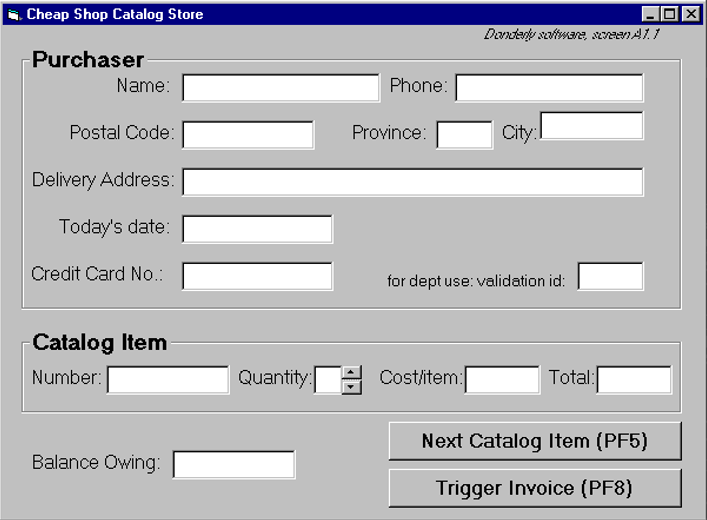
\includegraphics[width=0.7\textwidth]{28_Screen1.png} \par
    \vspace{3mm}
   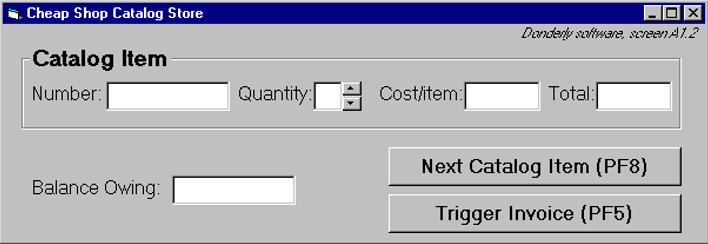
\includegraphics[width=0.7\textwidth]{28_Screen2.png}  
\end{wrapfigure}
\frametitle{\textcolor{myBlue}{\textbf{\hspace{5mm}{Cheap Shop}}}} \par
\vspace{10mm}
\textcolor{myBlue}{\footnotesize{{\hspace{15mm}{Screen 1}}}}\par
\vspace{40mm}
\textcolor{myBlue}{\footnotesize{{\hspace{15mm}{Screen 2}}}}
\end{frame}}



% Horodincă Alina-Elena
% slide 29
{%\setbeamercolor{background canvas}{bg=background}
\begin{frame}
\frametitle{\textcolor{myBlue}{\textbf{\hspace{8mm}{Specifications}}}}
\vspace*{-3mm}
\textcolor{red}{\rule{10cm}{1mm}}

\textcolor{myBlue}{\textbf{\footnotesize{\hspace{2mm}{To create an order}}}}
\begin{itemize}
\setlength{\itemindent}{0.5cm}
\setlength{\itemsep}{-0.5mm}
	\item[\textcolor{myBlue}{$\bullet$}]\textcolor{myBlue}{{\scriptsize On screen \#1, shoppers enter their personal information and their first order }}
   	\item[\textcolor{myBlue}{$\bullet$}]\textcolor{myBlue}{{\scriptsize text is entered via keyboard}}
	\item[\textcolor{myBlue}{$\bullet$}]\textcolor{myBlue}{{\scriptsize the tab or mouse is used to go between fields}}
\end{itemize} 

\textcolor{myBlue}{\textbf{\footnotesize{\hspace{2mm}{Further orders}}}}
\begin{itemize}
\setlength{\itemindent}{0.5cm}
	\item[\textcolor{myBlue}{$\bullet$}]\textcolor{myBlue}{{\scriptsize shoppers go to the 2nd screen by pressing the Next Catalog Item button}}
\end{itemize}

\textcolor{myBlue}{\textbf{\footnotesize{\hspace{2mm}{Order completion}}}}
\begin{itemize}
\setlength{\itemindent}{0.5cm}
\setlength{\itemsep}{-0.5mm}
	\item[\textcolor{myBlue}{$\bullet$}]\textcolor{myBlue}{{\scriptsize shoppers select ‘Trigger Invoice’. }}
    \item[\textcolor{myBlue}{$\bullet$}]\textcolor{myBlue}{{\scriptsize the system automatically tells shipping and billing about the order}}
	\item[\textcolor{myBlue}{$\bullet$}]\textcolor{myBlue}{{\scriptsize the system returns to a blank screen \#1}}
\end{itemize}

\textcolor{myBlue}{\textbf{\footnotesize{\hspace{2mm}{To cancel order}}}}
\begin{itemize}
\setlength{\itemindent}{0.5cm}
\setlength{\itemsep}{-0.5mm}
	\item[\textcolor{myBlue}{$\bullet$}]\textcolor{myBlue}{{\scriptsize Shoppers do not enter input for 30 seconds (as if they walk away)}}
    \item[\textcolor{myBlue}{$\bullet$}]\textcolor{myBlue}{{\scriptsize The system will then clear all screens and return to the main screen }}
\end{itemize} 

\textcolor{myBlue}{\textbf{\footnotesize{\hspace{2mm}{Input checking}}}}
\begin{itemize}
\setlength{\itemindent}{0.5cm}
\setlength{\itemsep}{-0.5mm}
	\item[\textcolor{myBlue}{$\bullet$}]\textcolor{myBlue}{{\scriptsize all input fields checked when either button is pressed.}}
	\item[\textcolor{myBlue}{$\bullet$}]\textcolor{myBlue}{{\scriptsize erroneous fields will blink for 3 seconds, and will then be cleared.}}
	\item[\textcolor{myBlue}{$\bullet$}]\textcolor{myBlue}{{\scriptsize the shopper can then re-enter the correct values in those fields.}}
\end{itemize}
\end{frame}}



% Horodincă Alina-Elena
% slide 30
{%\setbeamercolor{background canvas}{bg=background}
\begin{frame}
\frametitle{\textcolor{myBlue}{\textbf{\hspace{8mm}{Walkthrough template}}\textbf{\hspace{32mm}{{\small{\textsuperscript{\textcolor{black}{Task number: \underline{{ }{ }{ }{ }}}}}}}}}}
\vspace*{-2mm}
\textcolor{red}{\rule{11cm}{1mm}}
\begin{table}
\resizebox{\textwidth}{!}{%
\begin{tabular} { l |l | l | c }	
 	Description of 	& Does the user have the   &   Is it believable that they   &  Comment /  solution 	\\
  	Step           	& knowledge/training to do &   would do it?                 &                      	\\
   	               	& this?                    &   Are they motivated?          & 					  	\\
                   
  \hline
  
  					& 							& 								& 						\\ 
  					&							& 								& 						\\ 
   					& 							& 								& 						\\ 
  					&							& 								& 						\\ 
   					& 							& 								& 						\\ 
  					&							& 								& 						\\ 
   					& 							& 								& 						\\ 
  					&							& 								& 						\\ 
   					& 							& 								& 						\\ 
  					&							& 								& 						\\ 
   					& 							& 								& 						\\ 
  					&							& 								& 						\\  			
   					& 							& 								& 						\\ 
  					&							& 								& 						\\ 
   					& 							& 								& 						\\ 
  					&							& 								& 						\\ 
   					& 							& 								& 						\\ 
  					&							& 								& 						\\ 
\end{tabular}}
\end{table}
\fontsize{4pt}{5pt}\selectfont{ \textcolor{lightgray}{A walkthrough for this exercise is found in Greenberg, S. “Working through Task-Centered System Design. in Diaper, D. and Stanton, N. (Eds) The Handbook of Task Analysis for Human-Computer Interaction. Lawrence Erlbaum Associates}}
\end{frame}}



% Horodincă Alina-Elena
% slide 31
{%\setbeamercolor{background canvas}{bg=background}
\begin{frame}
\begin{wrapfigure}{r}{0.46\textwidth}
\vspace{27mm}
    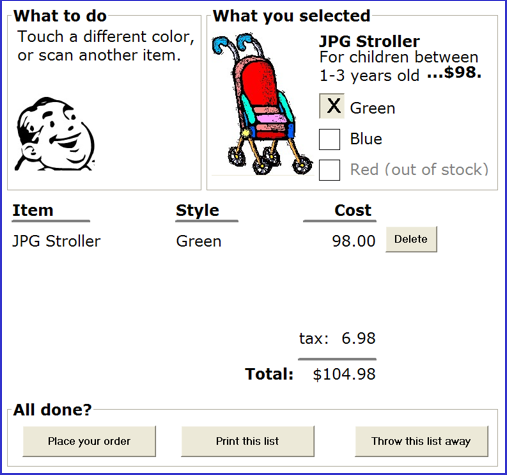
\includegraphics[width=0.55\textwidth]{31_Prototype.png} 
\end{wrapfigure}
\frametitle{\textcolor{myBlue}{\textbf{\hspace{8mm}{Are there better ways to do it?}}} }
\vspace*{-6mm}
\textcolor{red}{\rule{10cm}{1mm}} \par
\vspace{5mm}
\textcolor{myBlue}{\hspace{2mm}{A task-centered prototype}}
\begin{itemize}
	\item[\textcolor{myBlue}{--}] \textcolor{myBlue}{{\small partial wizard approach to tasks}}
    \item[\textcolor{myBlue}{--}] \textcolor{myBlue}{{\small prototyped several different ways}}
		\begin{itemize}
			\item[\textcolor{myBlue}{$\bullet$}]\textcolor{myBlue}{{\scriptsize paper - 45 minutes }}
         	\item[\textcolor{myBlue}{$\bullet$}]\textcolor{myBlue}{{\scriptsize scripted animation - 2 hours }}
		\end{itemize}    
\end{itemize}
	\vspace{25mm} 
\textcolor{myBlue}{\hspace{2mm}{Does it work?}}
\begin{itemize}
	\item[\textcolor{myBlue}{--}] \textcolor{myBlue}{{\small do a task-centered walkthrough to find out!}}
\end{itemize}
\end{frame}}



% Jurj Gheorghe Danut
% slide 32
{%\setbeamercolor{background canvas}{bg=background}
\begin{frame}{\LARGE{\bf{\color{myBlue}\hspace{6mm}Goal-centered system design}}}
\vspace*{-2mm}
{\textcolor{red}{\rule{11cm}{2.5pt}}}
\color{myBlue} {

{\Large Articulate user goals instead of task sequences}}
\bigskip
	\begin{itemize}
    \color{myBlue}
	\item[\textcolor{myBlue}{--}] Goal:
		\begin{itemize}
        \color{myBlue}
		\item[\textcolor{myBlue}{•}] a desired end condition
		\item[\textcolor{myBlue}{•}] tend to be stable
		\end{itemize}
    \bigskip
	\bigskip
	\item[\textcolor{myBlue}{--}] Task: 
		\begin{itemize}
        \color{myBlue}
		\item[\textcolor{myBlue}{•}] an intermediate process needed to achieve the goal
		\item[\textcolor{myBlue}{•}] may change as technology / work patterns change
        \end{itemize}
	\end{itemize}
    \bigskip \bigskip \bigskip \bigskip \bigskip \bigskip \bigskip
    %footer 
\leavevmode\makebox(0,0){\put(-25,0){\tiny{\textcolor{gray}{See Allan Cooper ‘The inmates are running the asylum’, Sams (Macmillan), especially Chapter 9 and 11.
}}}}
%\leavevmode\makebox(0,0){\put(280,0){\tiny{\textcolor{gray}{Saul Greenberg}}}}
\end{frame}


% Jurj Gheorghe Danut
% slide 33
\begin{frame} {\LARGE{\bf{\color{myBlue}\hspace{6mm}Goal-centered system design}}}
\vspace*{-2mm}
{\textcolor{red}{\rule{11cm}{2.5pt}}}
\color{myBlue}

\hspace{1mm}
\Large Designer
	\begin{itemize}
    \color{myBlue}
	\item[\textcolor{myBlue}{--}] \normalsize looking for solutions that satisfy these goals
	\item[\textcolor{myBlue}{--}] \normalsize task sequence may differ substantially from current process
    \end{itemize}
\bigskip
\color{myBlue}
\hspace{1mm}
\Large Approach:
	\begin{itemize}
    \color{myBlue}
	\item[\textcolor{myBlue}{--}] \normalsize Develop a \textbf{\textit{persona}}
		\begin{itemize}
        \color{myBlue}
		\item[\textcolor{myBlue}{•}] precise, specific description of the user and the goal they wish to accomplish 
		\item[\textcolor{myBlue}{•}] a pretend  user that are hypothetical archetypes of actual users
		\item[\textcolor{myBlue}{•}] discovered as a by-product of investigating the problem domain
		\end{itemize}
    \medskip
    \color{myBlue}
	\item[\textcolor{myBlue}{--}] \normalsize Develop a cast of characters
		\begin{itemize}
        \color{myBlue}
		\item[\textcolor{myBlue}{•}] 3 – 12 unique personas
		\item[\textcolor{myBlue}{•}] one will be the primary persona – the main focus of the design
        \end{itemize}
    \end{itemize}
%    \leavevmode\makebox(0,0){\put(280,0){\tiny{\textcolor{gray}{Saul Greenberg}}}}
\end{frame}

% Jurj Gheorghe Danut
% slide 34
\begin{frame} {\LARGE{\bf{\color{myBlue}\hspace{6mm}You know now}}}
\vspace*{-2mm}
{\textcolor{red}{\rule{11cm}{2.5pt}}}
\color{myBlue}

\hspace{3mm}
\Large How to develop concrete task examples \par
\bigskip
\hspace{3mm}
\Large How to use task examples to motivate your designs \par 
\bigskip
\hspace{3mm}
\Large How to evaluate designs through task-centered walkthroughs \par
\bigskip \bigskip \bigskip \bigskip \bigskip \bigskip \bigskip \bigskip
%\leavevmode\makebox(0,0){\put(280,0){\tiny{\textcolor{gray}{Saul Greenberg}}}}
\end{frame}
}

% Jurj Gheorghe Danut
% slide 35
\begin{frame} {\bf{\color{myBlue}\hspace{6mm}Interface Design and Usability Engineering}}
\vspace*{-2mm}
{\textcolor{red}{\rule{11cm}{2.5pt}}}

\begin{figure}[h] \begin{flushright}
	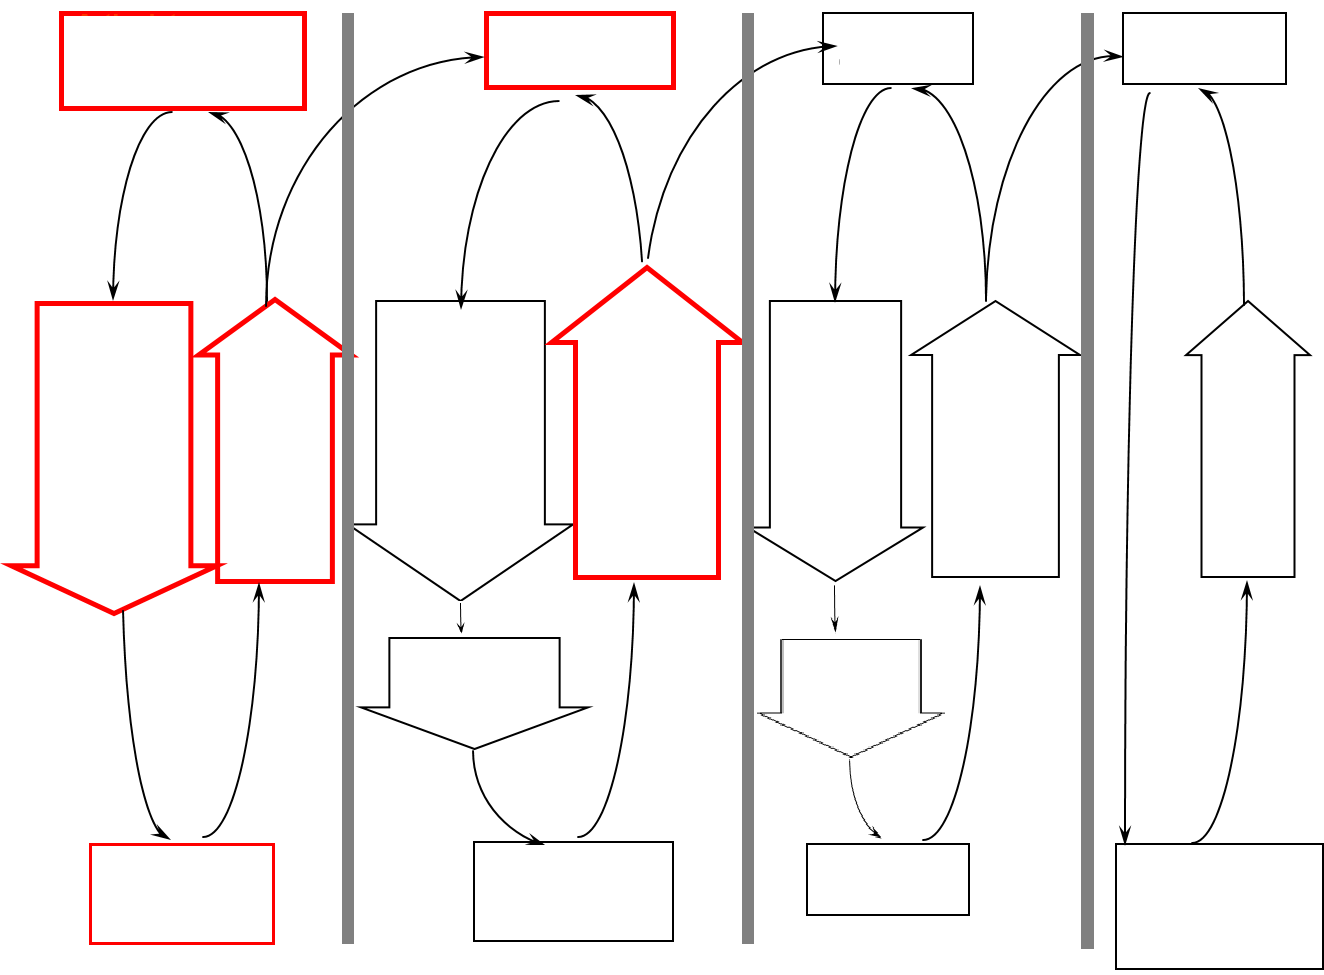
\includegraphics[width=0.98\textwidth]{35_schema.png}
\end{flushright}
\end{figure}
\leavevmode\makebox(0,0){\put(-27,450){\selectfont{\textbf{\footnotesize Goals:}}}}
\leavevmode\makebox(0,0){\put(-30,280){\selectfont{\textbf{\footnotesize Methods:}}}}
\leavevmode\makebox(0,0){\put(-33,80){\selectfont{\textbf{\footnotesize Products:}}}}
%prima coloana
\leavevmode\makebox(0,0){\put(10,470){\selectfont{\textbf{\tiny \color{orange} Articulate:}}}}
\leavevmode\makebox(0,0){\put(9,460){\selectfont{\textbf{\tiny \color{orange} *who users are}}}}
\leavevmode\makebox(0,0){\put(5,450){\selectfont{\textbf{\tiny \color{orange} *their key tasks }}}}
\leavevmode\makebox(0,0){\put(-3,332){\selectfont{\textbf{\tiny \color{orange} Task }}}}
\leavevmode\makebox(0,0){\put(-7,320){\selectfont{\textbf{\tiny \color{orange} centered }}}}
\leavevmode\makebox(0,0){\put(-10,307){\selectfont{\textbf{\tiny \color{orange} system }}}}
\leavevmode\makebox(0,0){\put(-14,295){\selectfont{\textbf{\tiny \color{orange} design }}}}
\leavevmode\makebox(0,0){\put(-23,275){\selectfont{\tiny \textcolor{gray} {Participatory} }}}
\leavevmode\makebox(0,0){\put(-20,265){\selectfont{\tiny \textcolor{gray} {design} }}}
\leavevmode\makebox(0,0){\put(-25,250){\selectfont{\tiny \textcolor{gray} {User-} }}}
\leavevmode\makebox(0,0){\put(-28,240){\selectfont{\tiny \textcolor{gray} {centered} }}}
\leavevmode\makebox(0,0){\put(-32,230){\selectfont{\tiny \textcolor{gray} {design} }}}
\leavevmode\makebox(0,0){\put(-27,80){\selectfont{\textbf{\tiny \color{orange} User and task }}}}
\leavevmode\makebox(0,0){\put(-26,70){\selectfont{\textbf{\tiny \color{orange} description }}}}
\leavevmode\makebox(0,0){\put(-5,280){\selectfont{\textbf{\tiny \color{orange} Evaluate }}}}
\leavevmode\makebox(0,0){\put(-8,265){\selectfont{\textbf{\tiny \color{orange} tasks }}}}
%a doua coloana
\leavevmode\makebox(0,0){\put(50,470){\selectfont{\textbf{\tiny \color{orange} Brainstorm }}}}
\leavevmode\makebox(0,0){\put(48,460){\selectfont{\textbf{\tiny \color{orange} design }}}}
\leavevmode\makebox(0,0){\put(15,330){\selectfont{\textcolor{gray}{\tiny Psychology of }}}}
\leavevmode\makebox(0,0){\put(12,320){\selectfont{\textcolor{gray}{\tiny everyday }}}}
\leavevmode\makebox(0,0){\put(8,310){\selectfont{\textcolor{gray}{\tiny things }}}}
\leavevmode\makebox(0,0){\put(5,290){\selectfont{\textcolor{gray}{\tiny User }}}}
\leavevmode\makebox(0,0){\put(2,280){\selectfont{\textcolor{gray}{\tiny involvement }}}}
\leavevmode\makebox(0,0){\put(-3,260){\selectfont{\textcolor{gray}{\tiny Representation }}}}
\leavevmode\makebox(0,0){\put(-4,250){\selectfont{\textcolor{gray}{\tiny metaphors }}}}
\leavevmode\makebox(0,0){\put(-5,180){\selectfont{\textcolor{gray}{\tiny low fidelity }}}}
\leavevmode\makebox(0,0){\put(-8,170){\selectfont{\textcolor{gray}{\tiny prototyping }}}}
\leavevmode\makebox(0,0){\put(-11,160){\selectfont{\textcolor{gray}{\tiny methods }}}}
\leavevmode\makebox(0,0){\put(5,90){\selectfont{\textcolor{gray}{\tiny Throw-away }}}}
\leavevmode\makebox(0,0){\put(2,80){\selectfont{\textcolor{gray}{\tiny paper }}}}
\leavevmode\makebox(0,0){\put(-1,70){\selectfont{\textcolor{gray}{\tiny prototypes }}}}
\leavevmode\makebox(0,0){\put(13,320){\selectfont{\textcolor{gray}{\tiny Participatory }}}}
\leavevmode\makebox(0,0){\put(10,310){\selectfont{\textcolor{gray}{\tiny interaction }}}}
\leavevmode\makebox(0,0){\put(7,280){\selectfont{\textbf{\tiny \color{orange} Task }}}}
\leavevmode\makebox(0,0){\put(5,270){\selectfont{\textbf{\tiny \color{orange} scenario }}}}
\leavevmode\makebox(0,0){\put(1,260){\selectfont{\textbf{\tiny \color{orange} walk- }}}}
\leavevmode\makebox(0,0){\put(-2,250){\selectfont{\textbf{\tiny \color{orange} through }}}}
%a treia coloana
\leavevmode\makebox(0,0){\put(52,470){\selectfont{\textcolor{gray}{\tiny Redefined }}}}
\leavevmode\makebox(0,0){\put(49,460){\selectfont{\textcolor{gray}{\tiny designs }}}}
\leavevmode\makebox(0,0){\put(30,340){\selectfont{\textcolor{gray}{\tiny Graphical }}}}
\leavevmode\makebox(0,0){\put(30,330){\selectfont{\textcolor{gray}{\tiny screen }}}}
\leavevmode\makebox(0,0){\put(25,320){\selectfont{\textcolor{gray}{\tiny design }}}}
\leavevmode\makebox(0,0){\put(20,300){\selectfont{\textcolor{gray}{\tiny Interface }}}}
\leavevmode\makebox(0,0){\put(15,290){\selectfont{\textcolor{gray}{\tiny guidelines }}}}
\leavevmode\makebox(0,0){\put(13,270){\selectfont{\textcolor{gray}{\tiny Style }}}}
\leavevmode\makebox(0,0){\put(10,260){\selectfont{\textcolor{gray}{\tiny guides }}}}
\leavevmode\makebox(0,0){\put(5,180){\selectfont{\textcolor{gray}{\tiny high fidelity }}}}
\leavevmode\makebox(0,0){\put(2,170){\selectfont{\textcolor{gray}{\tiny prototyping }}}}
\leavevmode\makebox(0,0){\put(-1,160){\selectfont{\textcolor{gray}{\tiny methods }}}}
\leavevmode\makebox(0,0){\put(5,90){\selectfont{\textcolor{gray}{\tiny Testable }}}}
\leavevmode\makebox(0,0){\put(2,80){\selectfont{\textcolor{gray}{\tiny prototypes }}}}
\leavevmode\makebox(0,0){\put(23,320){\selectfont{\textcolor{gray}{\tiny Usability }}}}
\leavevmode\makebox(0,0){\put(20,310){\selectfont{\textcolor{gray}{\tiny testing }}}}
\leavevmode\makebox(0,0){\put(15,280){\selectfont{\textcolor{gray}{\tiny Heuristic }}}}
\leavevmode\makebox(0,0){\put(12,270){\selectfont{\textcolor{gray}{\tiny evaluation }}}}
%a patra coloana
\leavevmode\makebox(0,0){\put(55,470){\selectfont{\textcolor{gray}{\tiny Completed }}}}
\leavevmode\makebox(0,0){\put(52,460){\selectfont{\textcolor{gray}{\tiny designs }}}}
\leavevmode\makebox(0,0){\put(65,310){\selectfont{\textcolor{gray}{\tiny Field }}}}
\leavevmode\makebox(0,0){\put(60,300){\selectfont{\textcolor{gray}{\tiny testing }}}}
\leavevmode\makebox(0,0){\put(40,90){\selectfont{\textcolor{gray}{\tiny Alpha/beta }}}}
\leavevmode\makebox(0,0){\put(36,80){\selectfont{\textcolor{gray}{\tiny systems or }}}}
\leavevmode\makebox(0,0){\put(33,70){\selectfont{\textcolor{gray}{\tiny complete }}}}
\leavevmode\makebox(0,0){\put(29,60){\selectfont{\textcolor{gray}{\tiny specification }}}}
\end{frame}



\setbeamercolor{normal text}{fg=Blue}
\usebeamercolor[fg]{normal text}
\begin{frame}
	\vspace{8mm}
	\textcolor{Blue}{\textbf{\Large{*Bibliography}}}
    \textcolor{red}{\rule{10cm}{1mm}}

    \begin{itemize}
    	\item[] 
        \begin{itemize}
        	\item[{$\bullet$}] Saul Greenberg, \textbf{Understanding users and their tasks. Task-centered system design }, University of Calgary, Canada

        	\url{http://pages.cpsc.ucalgary.ca/~saul/481/}
\newline        	
	
        	\item[{$\bullet$}] Saul Greenberg, \textbf{Working through Task-Centered System Design}, in Diaper, D. and Stanton, N. (Eds) The Handbook of Task Analysis for Human-Computer Interaction, Lawrence Erlbaum Associates, pp. 49-66
        	
        	\url{http://www.hcitang.org/uploads/Teaching/481-reading-working-through-task-centered-system-design.pdf}
\newline

        	\item[{$\bullet$}] Keith Andrews, \textbf{Human Computer Interaction, Chapter 4. User Research \& Chapter 6. Interaction Design}, TU Graz, Austria

        	\url{https://courses.isds.tugraz.at/hci/hci.pdf}        	
     	\end{itemize}
   	\end{itemize}
\end{frame}



\end{document}